\IEEEPARstart{W}{e} present our results with two Intel target architectures - Xeon E-2278G and Xeon E5-1650v4. Both architectures run AlmaLinux 8.5, where we have performed our experiments. Table 4.1 highlights the CPU properties. We use Intel compiler ICC 19.1.3.304 with -O3  -qopenmp -xCORE-AVX2 -ipo options as a compiler flag.

\begin{table}[htbp]
\caption{\uppercase{CPU Parameters Overview}}
\label{tab:cpu parameters}
\begin{center}
\begin{tabular}{|c||c|c|}
\hline
 Parameters & Xeon E5-1650v4  & Xeon E-2278G \\
\hline
\hline
Micro-Architecture & Broadwell  & Coffee Lake \\
\hline
Number of cores & 6 & 8  \\
Number of threads & 12 & 16  \\
\hline
Base Frequency (GHz) & 3.6  & 3.4  \\
Turbo Frequency (GHz) & 4.0 & 5.0   \\
\hline
L1 Cache (KB) - Per Core  & 32 & 32  \\
L2 Cache (KB) - Per Core &  256  & 256 \\
L3 Cache (MB) - Shared & 15 & 16 \\
DRAM (GB) & 16 & 32 \\
\hline
\end{tabular}
\end{center}
\end{table}


Our optimized BPMax uses single-precision floating point. We measure the performance by calculating the number of single-precision floating-point operations executed per second (FLOPS). Now, GFLOPS indicates $10^9$ floating-point operations per second. Although GFLOPS is typically used to highlight double-precision performance, we will use this terminology to denote the single-precision performance in the rest of our discussion. We first present the theoretical machine peak, then the Roofline machine peak measured by the Intel Advisor before presenting the Double max-plus and BPMax performance.

\subsection{Max-plus Machine Peak Analysis}
We calculate the theoretical CPU machine peak using the following equation:
\begin{equation}\label{eqn:machine_peak_eqn}
\begin{split}
\text{Single-precision Machine Peak (GFLOPS)} &= \\
\text{Number of vector operations} \times \text {Instructions per cycle} \times \\
\text{Number of Cores} \times \text{Core Frequency (GHz)} \\
\end{split}
\end{equation}


Table~\ref{tab1:Theoretical_machine_peak} highlights the theoretical machine peak of our target architectures. Coffee Lake and Broadwell's theoretical max-plus machine peaks are $435.2$ and $172$ GFLOPS, respectively, when the cores run at the base frequency.

\begin{table*}[htbp]
\caption{\uppercase{Max-plus Theoretical Machine Peak}}
\label{tab1:Theoretical_machine_peak}
\begin{center}
\begin{tabular}{|c|c|c|c|c|c|}
\hline
 & Number &  Frequency &  Instructions & Machine Peak Single Core (GFLOPS)& Machine Peak Total\\
 Processor & of Cores& (GHz)  & per cycle & (GFLOPS) & (GFLOPS)\\
  & &  [Base, Turbo] & [add, max]  & [Base, Turbo] & [Base, Turbo]\\
\hline
Xeon E5-1650v4 & 6 & [3.6, 4.0] & [1, 1] & [28.8, 32] & [172.8, 192] \\
\hline
Xeon E-2278G & 8 & [3.4, 5.0] & [2, 2] & [54.4, 80] & [435.2, 640] \\
\hline
%\multicolumn{5}{l}{}
\end{tabular}
\end{center}
\end{table*}


\textbf{Arithmetic Intensity of BPMax:} BPMax computation can be summarized as $ Y = max(a + X, Y)$.  It uses three single-precision memory accesses to perform two arithmetic operations (max and plus). So, its arithmetic intensity (AI) is $\frac{2}{(3\times4)}$or $\frac{1}{6}$ FLOPS/byte.

\textbf{Coffee Lake Roofline}: Figure~\ref{fig:roof_line_coffee_lake} shows the max-plus Roofline collected on the Coffee Lake machine using the Intel Advisor tool. We observe that the attainable max-plus machine peak of Coffee Lake in our environment is around 585 GFLOPS, which is significantly lower than the theoretical max-plus machine peak of 640 GLOPS with the processor running at maximum frequency.

\begin{figure}[htbp]
\centerline{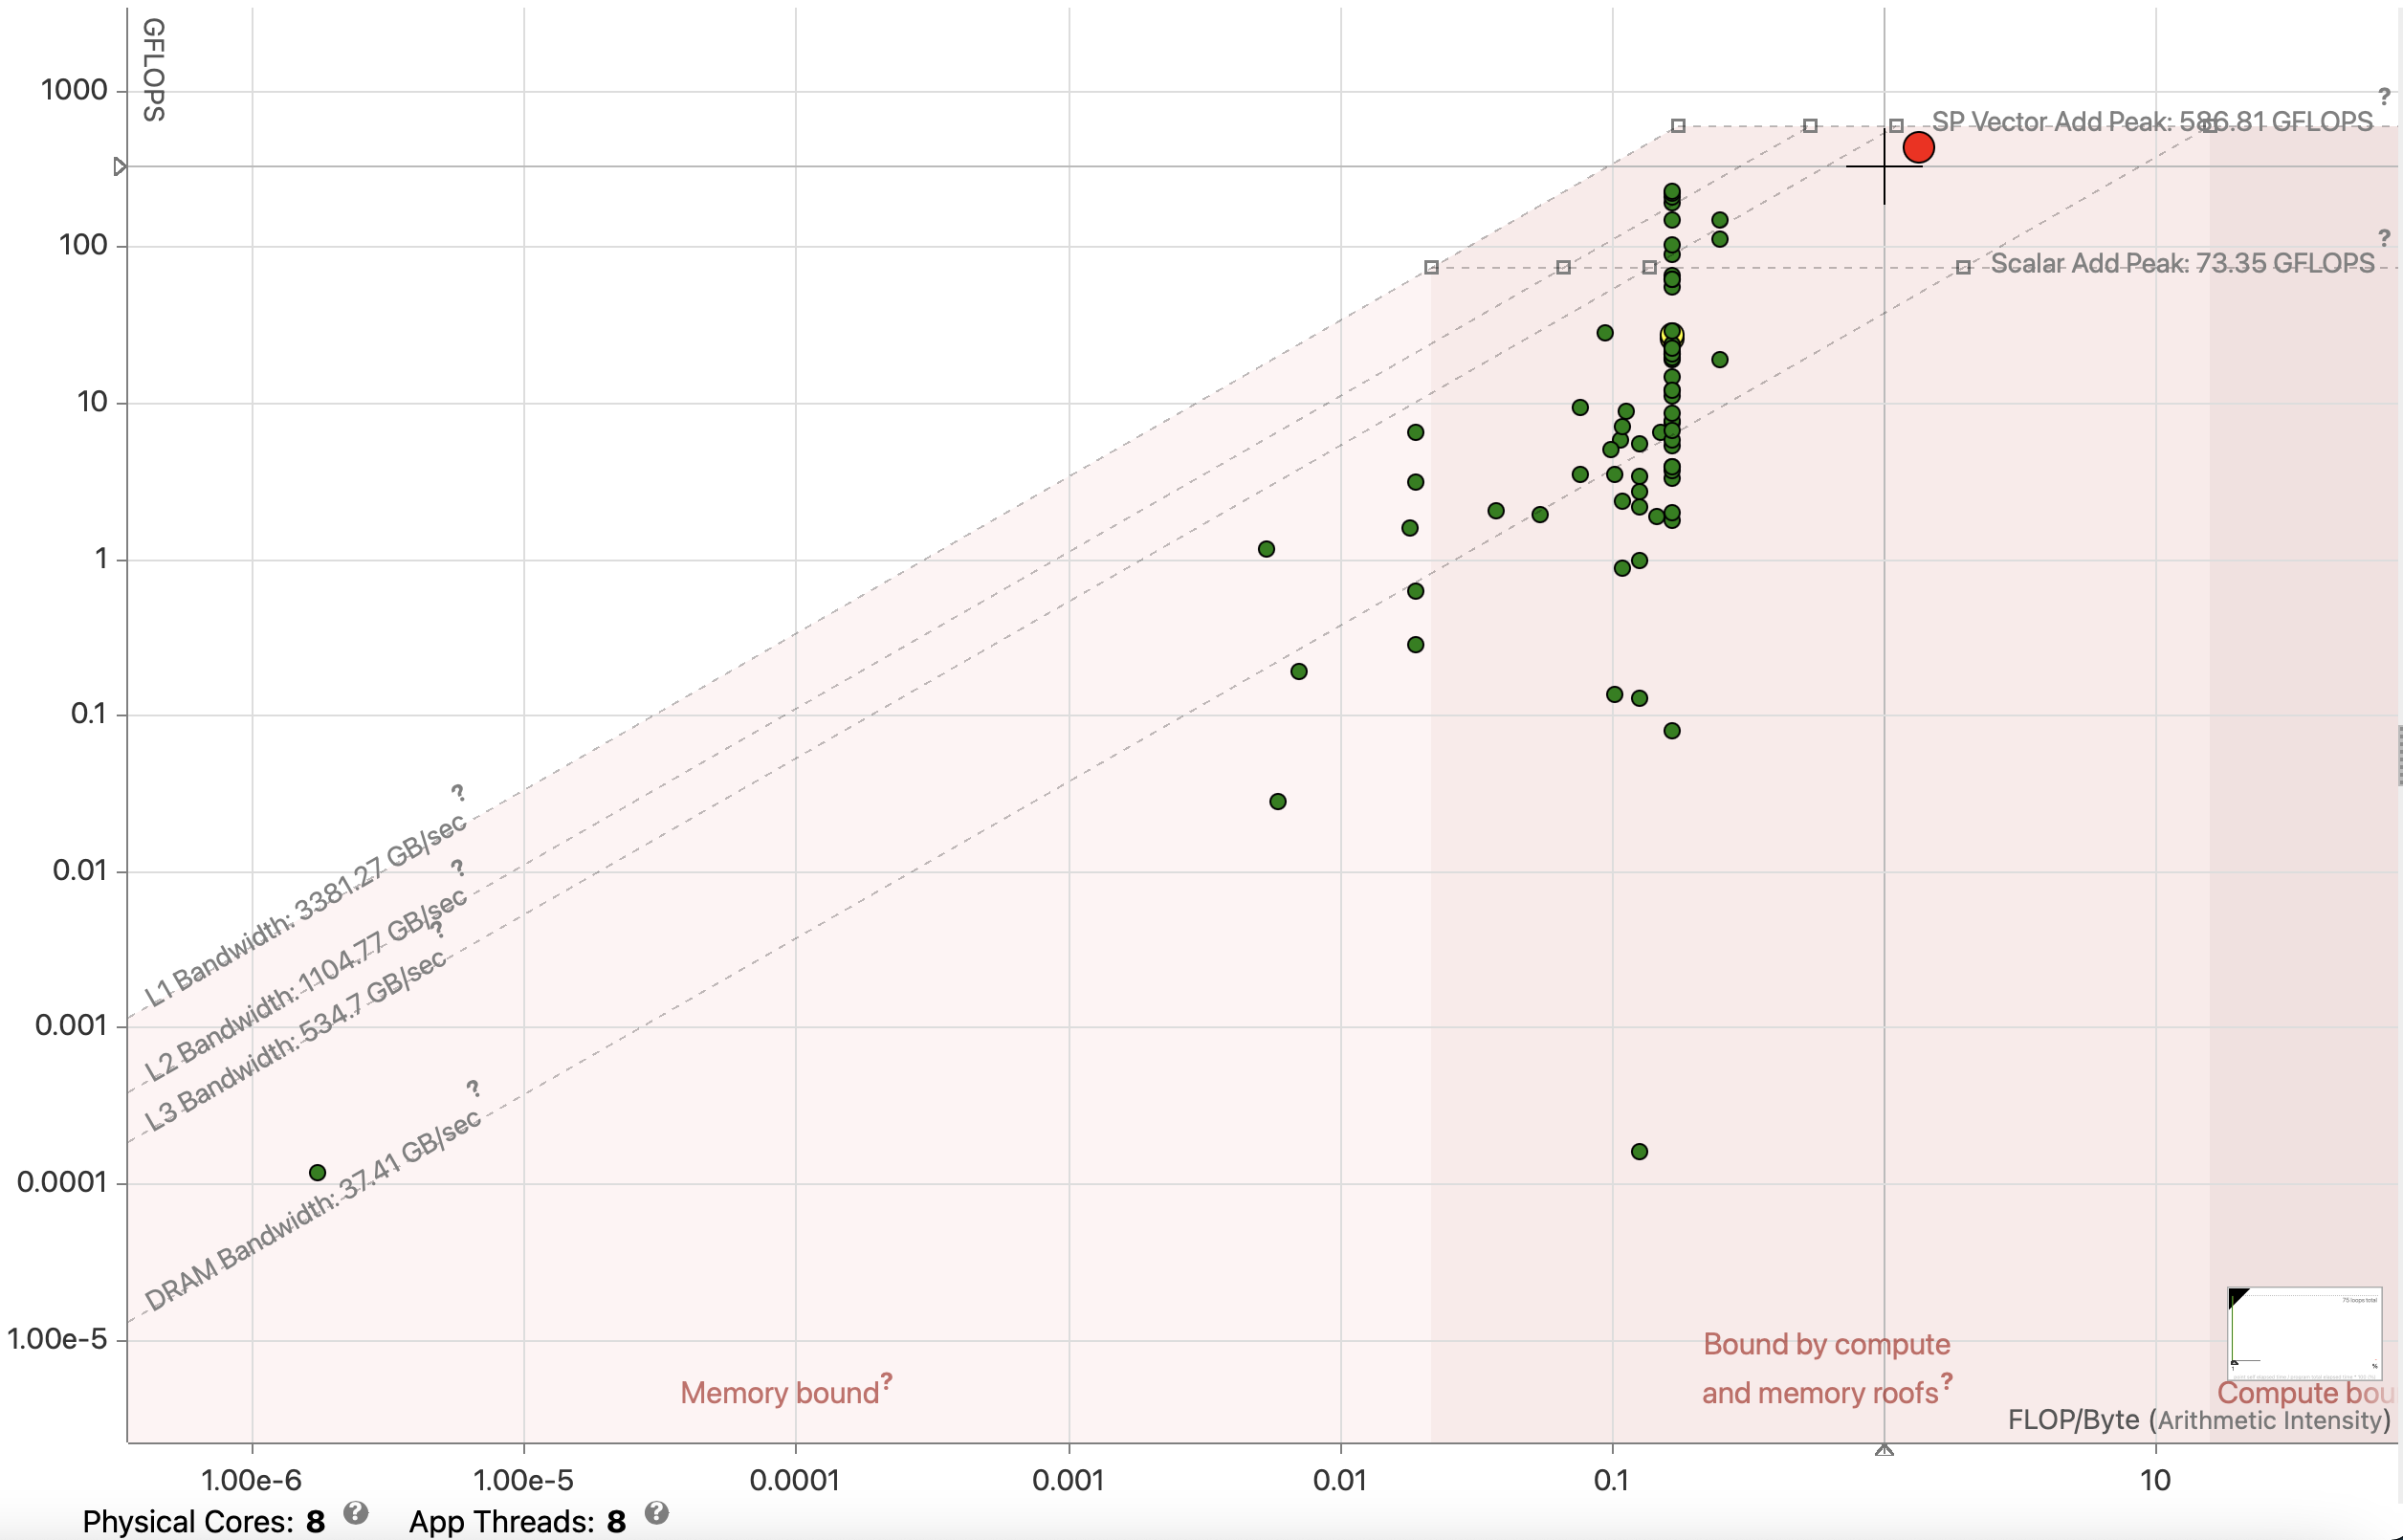
\includegraphics[scale=0.20, trim=0 0 0 0,clip]{content/figures/roofline_coffee_lake.png}}
\caption{Xeon E-2278G (Coffee Lake) roofline for max-plus}
\label{fig:roof_line_coffee_lake}
\end{figure}


{\textbf{Broadwell Roofline:}} Figure~\ref{fig:roof_line_broad_well} presents the Broadwell's Roofline model. From this Roofline model, we observe that Broadwell's attainable max-plus machine peak is around 165 GFLOPS, which is $85\%$ of the theoretical machine peak (192 GFLOPS), with the processor running at maximum frequency.

\begin{figure}[htbp]
\centerline{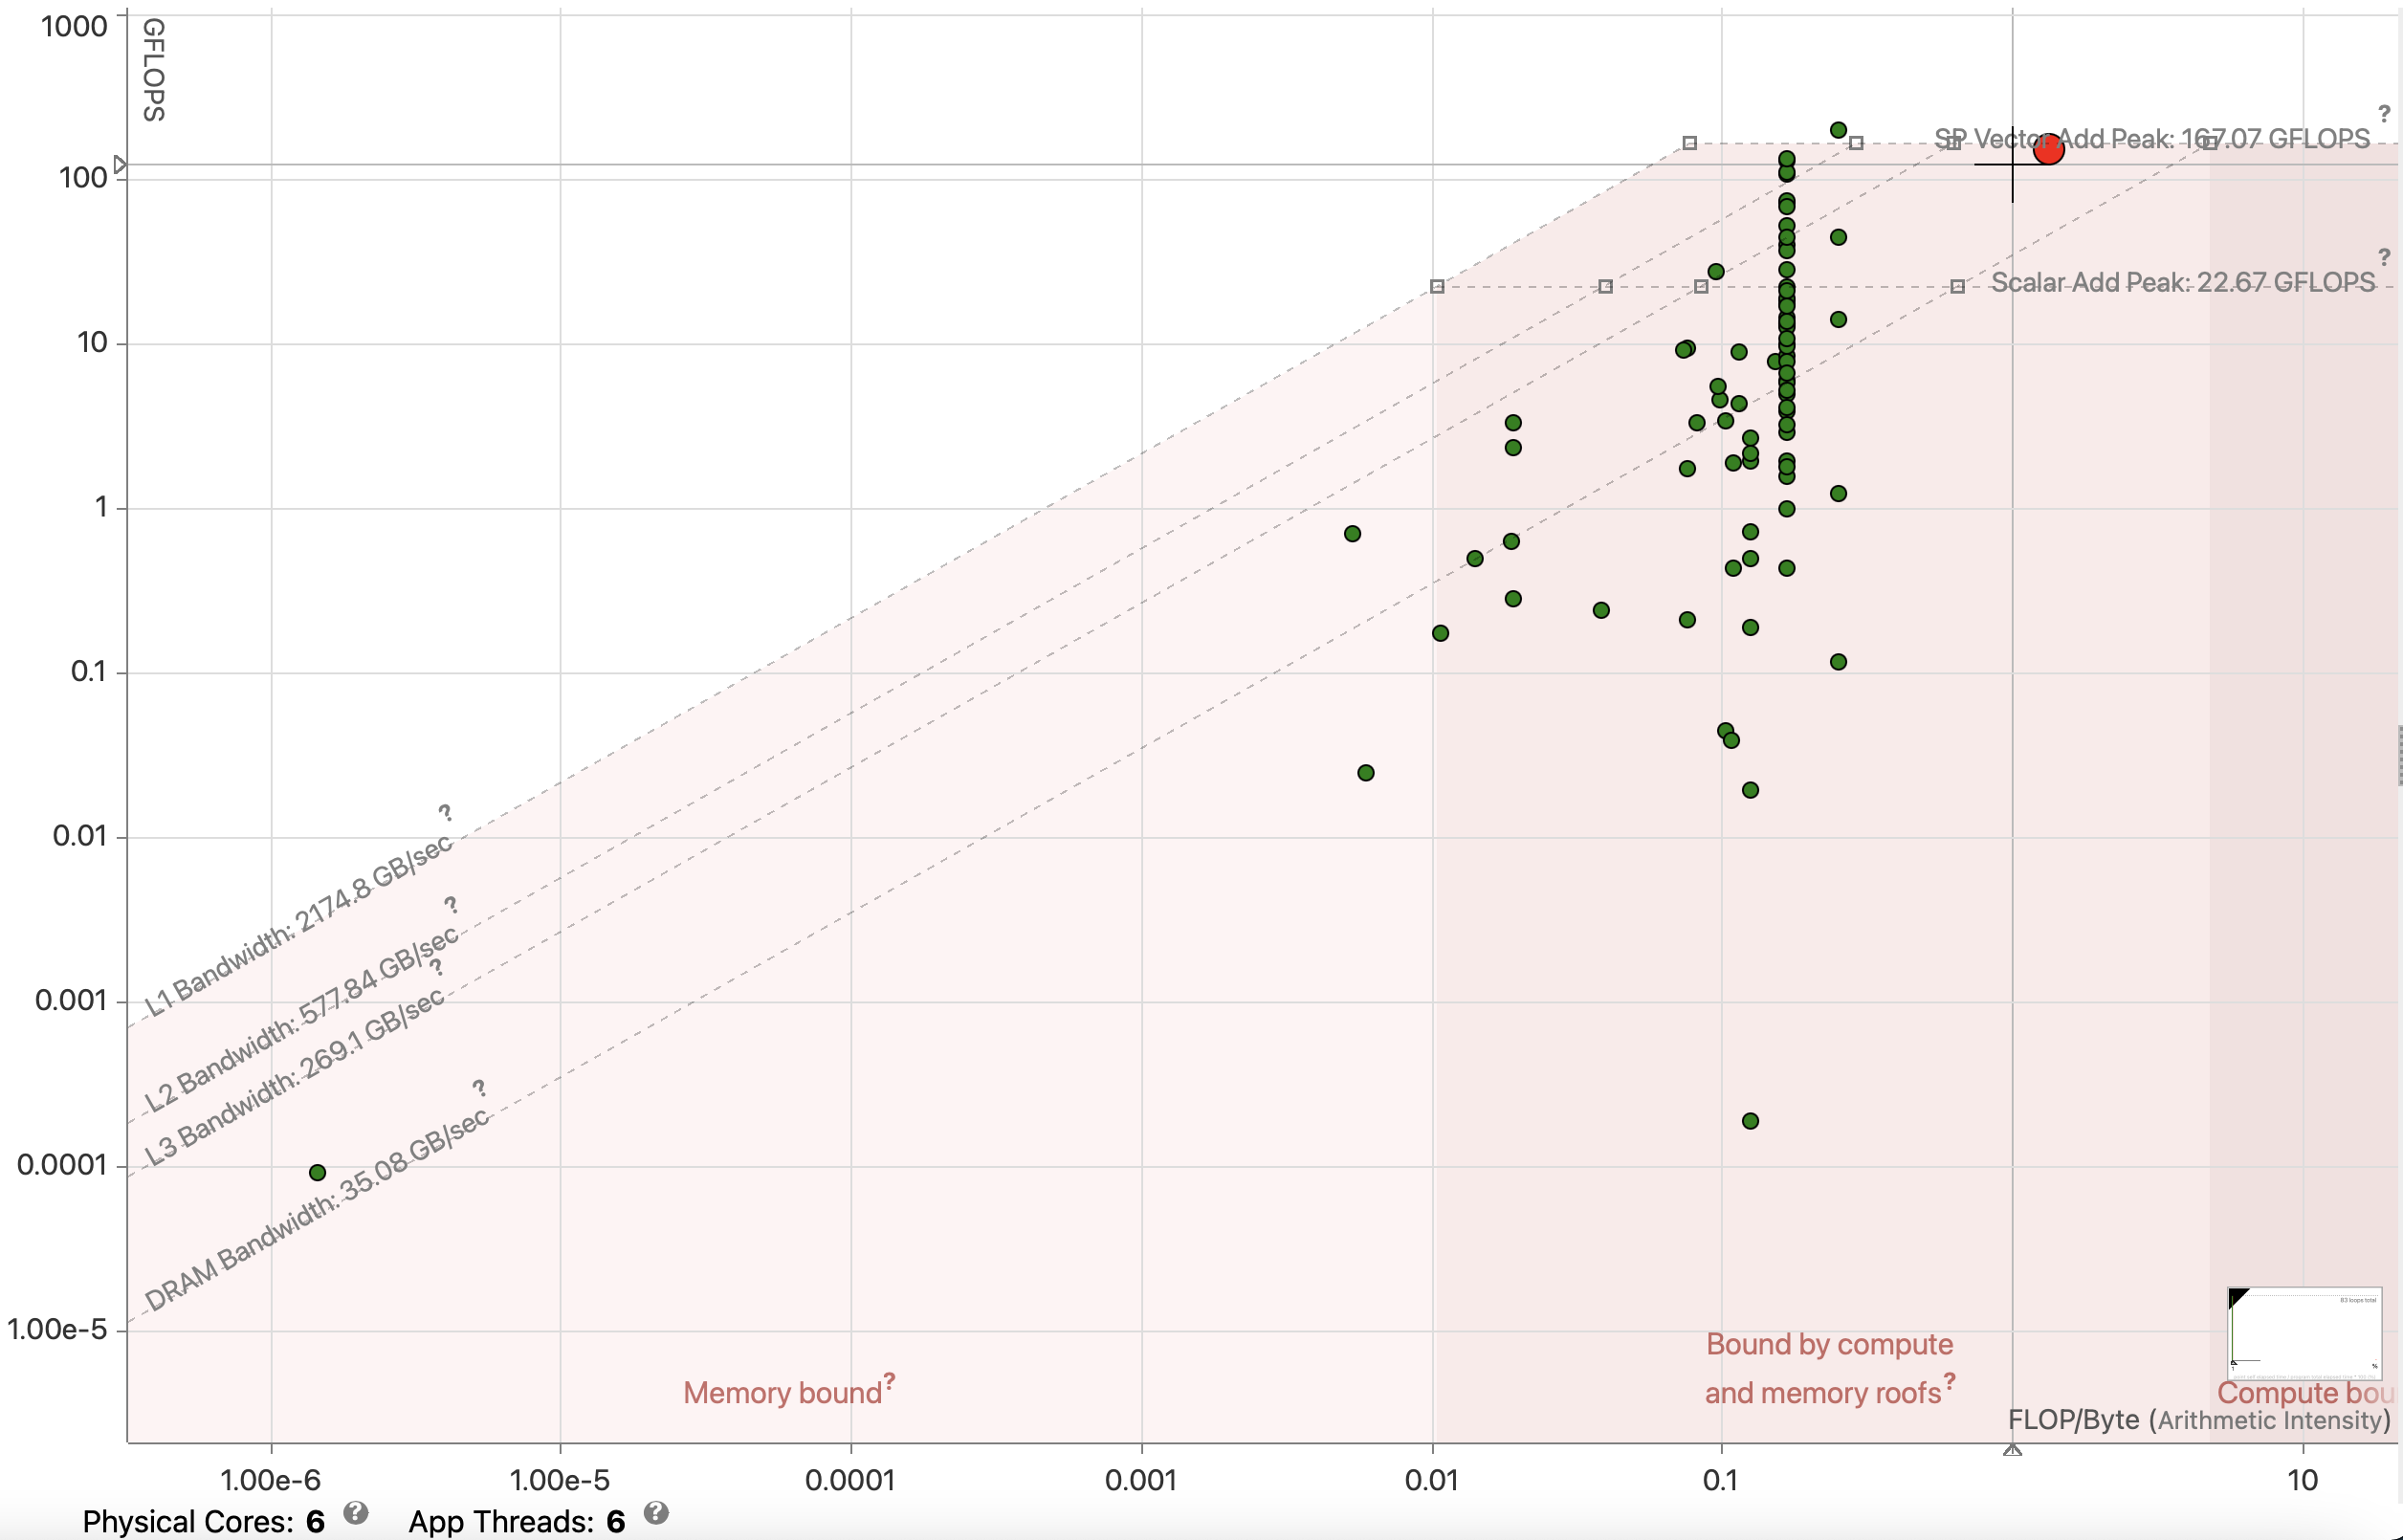
\includegraphics[scale=0.20, trim=0 0 0 0,clip]{content/figures/roofline_broadwell.png}}
\caption{Xeon E5 1650v4 (Broadwell) Roofline for max-plus}
\label{fig:roof_line_broad_well}
\end{figure}


\subsubsection{Tile Parameter Exploration}
We use three levels of tiling (Fig~\ref{fig:bpmax_full_tiling}) in our optimization. The size of the first-level tile depends on the length of the second input sequence($N$), which is a program parameter. That leaves us to explore second and third-level tiling parameters. We have implemented a micro-kernel that performs matrix-max plus operation on two square matrices of size ($N \times N$) to explore the best register tile and mono-parametric tile parameter. We choose square matrices $(N = 2800)$ such that the footprint exceeds the L3 cache. Figure~\ref{fig:register_tile_performance_comparison} compares performance between different register tiles on Coffee Lake. We tile the three outer loops with a mono-parametric tile size of $192$. Then, we register-tile each patch. The register-tile kernel assumes that the data is accessed sequentially. All the results shown here include the packing operation of these patches.
\begin{figure}[htbp]
    \centering
    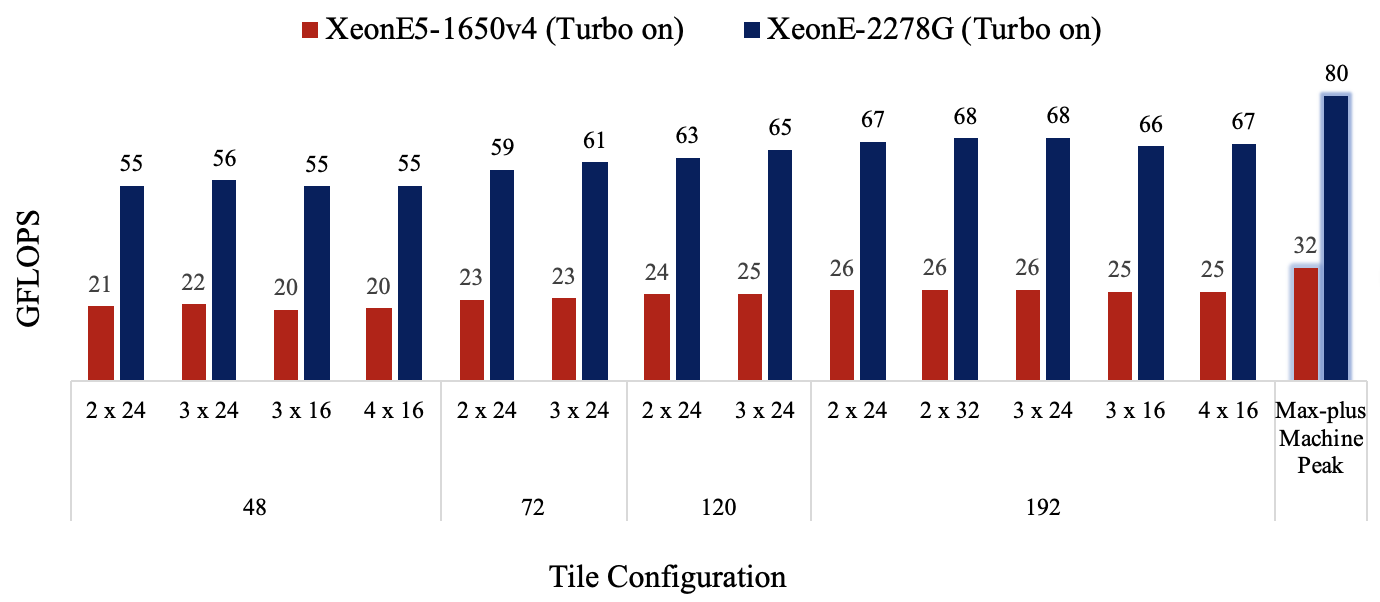
\includegraphics[scale=0.37, trim=4 4 4 4,clip]{content/figures/max_plus_register_tile_performance_new.png}
   \caption{Register-Tiled Max-plus Performance}
\label{fig:register_tile_performance_comparison}
\end{figure}
We notice that the register-tile $3 \times 24$ performs the best which matches our theoretical register allocation strategy. 
To explore second-level tile size, we fixed the register tile parameters and vary the second-level tile size [48, 72, 120, 192]. We find that the second-level tile size of 48 performs better than the others for double max-plus and BPMax when the register-tile size is $3 \times 24$. When $N_{tile}=48$, all the inputs and outputs of the register-tiled kernel fit in the $L_{1}$. So, we use $N_{tile}=48$ and the register-tile dimension of $3 \times 24$ for the rest of our experiments.



\subsection{Double Max-plus Performance Improvement}
\subsubsection{Single Core Performance}
Figure~\ref{fig:st_performance_analysis_double_max_plus} presents the performance of the double max-plus on a single thread of Xeon E5-1650v4 (Broadwell) and Xeon E-2278G (Coffee Lake). We compare the performance between the best optimized previous version ~\cite{Mondal2021} and the current version with the diagonal schedule.
\begin{figure}[htbp]
\centerline{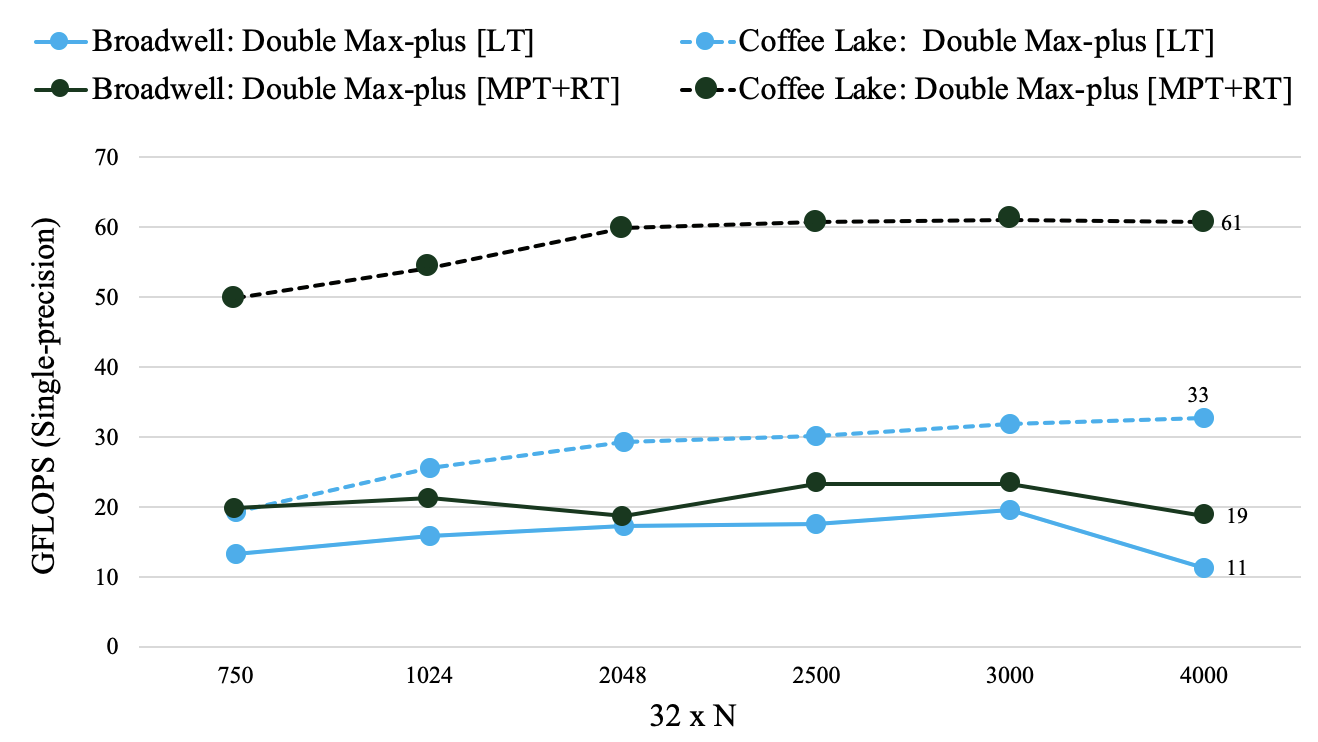
\includegraphics[scale=0.38, trim=5 5 5 5,clip]{content/figures/dpm_single_core_new.png}}
\caption{Double Max-plus Single Core Performance}
\label{fig:st_performance_analysis_double_max_plus}
\end{figure}
Figure~\ref{fig:st_performance_analysis_double_max_plus} shows the performance of the double max-plus computation with these two versions of the code when $M$ is fixed to $32$ and $N$ is varied between $750$ to $4000$. We have not presented the base version since it only attains a tiny fractional GFLOPS performance. The previous best-optimized version of the program highlighted in sky-blue reaches about $50\%$ of the Roofline machine peak on both Broadwell (dotted blue line) and Coffee Lake (dotted dark-green line), whereas the current best-optimized version attains over $90\%$ and $80\%$ of the max-plus roofline machine peak on Broadwell (dark-green continuous line) and Coffee Lake (dark-green dotted line), respectively. Both program versions performed poorly on Broadwell when $N$ was larger than $3000$. It is due to the $F$-Table memory footprint becoming close to Broadwell's DRAM capacity (16 GB) when $M=32$, $N=4000$, triggering swapping (disk-access) that reduces CPU resource utilization. We do not see this behavior on Coffee Lake.


\subsubsection{Multi-Core Performance Comparison}
For our experiments on multi-core, we choose three different values of $M$ ($16$, $25$, $32$) and five different values of $N$ ($750$, $1024$, $2048$, $2500$, $3000$) to measure the double max-plus performance for each combination of $M$ and $N$. Figure~\ref{fig:peroformance_analysis_double_max_plus} and Figure~\ref{fig:double_max_plus_speed_up} show the performance and speedup comparisons of double max-plus between the base schedule, previously optimized best version ([LT]), and current best-optimized version ([MPT+RT]) with eight threads on Coffee Lake. The performance of the original code is about 1 GFLOPS, highlighted in dark red.
\begin{figure}[htbp]
\centerline{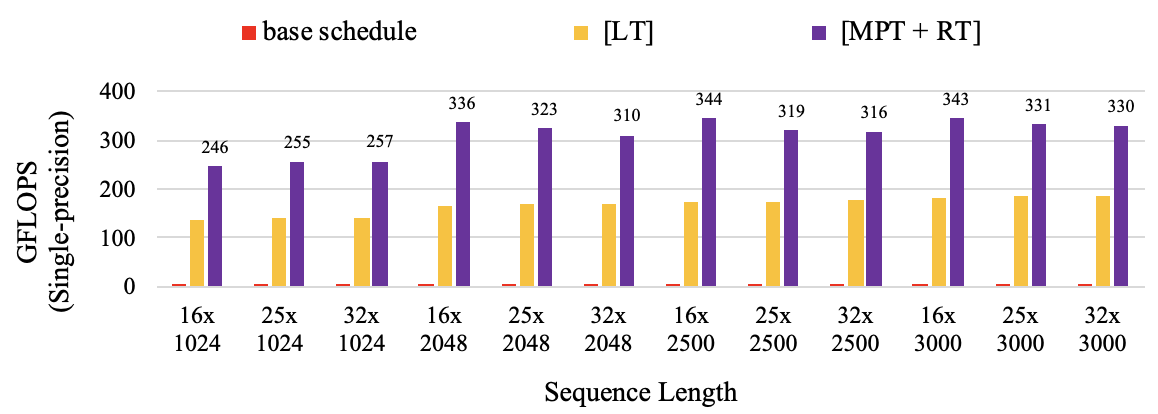
\includegraphics[scale=0.42, trim=5 5 5 5,clip]{content/figures/dpm_performance_new.png}}
\caption{Double Max-plus Performance, Coffee Lake }
\label{fig:peroformance_analysis_double_max_plus}
\end{figure}
\begin{figure}[htbp]
\centerline{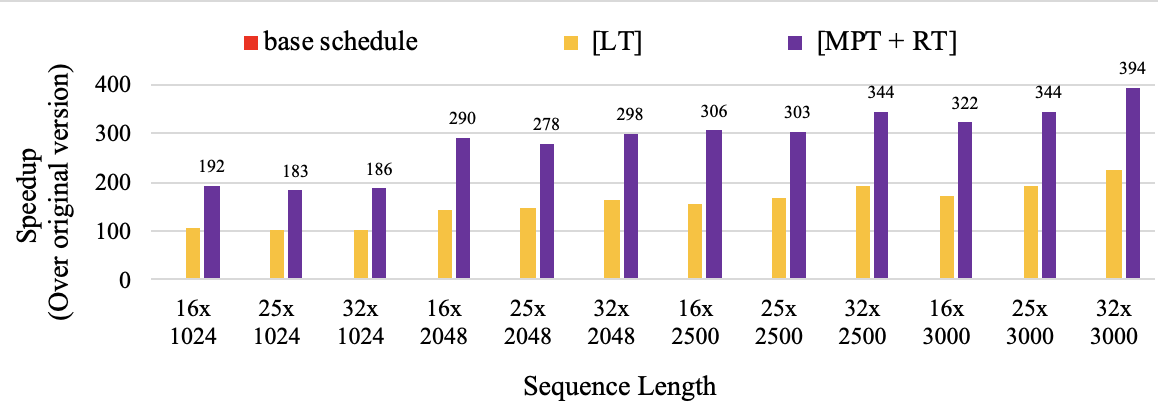
\includegraphics[scale=0.42, trim=5 5 5 5,clip]{content/figures/dpm_speedup_new.png}}
\caption{Double Max-plus Speedup, Coffee Lake}
\label{fig:double_max_plus_speed_up}
\end{figure}
The yellow color represents the performance corresponding to the [LT]. It attains a maximum performance of $187$ GFLOPS (32\% of the Roofline machine peak) on Coffee Lake. The best [MPT+RT] version, represented by the purple color, reaches a peak performance of $344$ GFLOPS, which is 58\% of the Roofline machine peak. These correspond to a speedup of $223\times$ and $394\times$  over the implementation available in the original BPMax program.




\subsection{BPMax Performance Improvement}
We have chosen input parameters similar to Double max-plus to measure the BPMax performance.

\subsubsection{Single-Core Performance}
Figure~\ref{fig:st_performance_analysis_bpmax} shows the single core performance of the best BPMax version, \textbf{[MPT+RT]:v3} with $M=32$ and $N$ varying between ($750$, $1024$, $2048$, $2500$, $3000$, $4000$). We attain about 80\% and 85\% of the roofline max-plus machine peak on Coffee Lake and Broadwell, respectively.
\begin{figure}[htbp]
\centerline{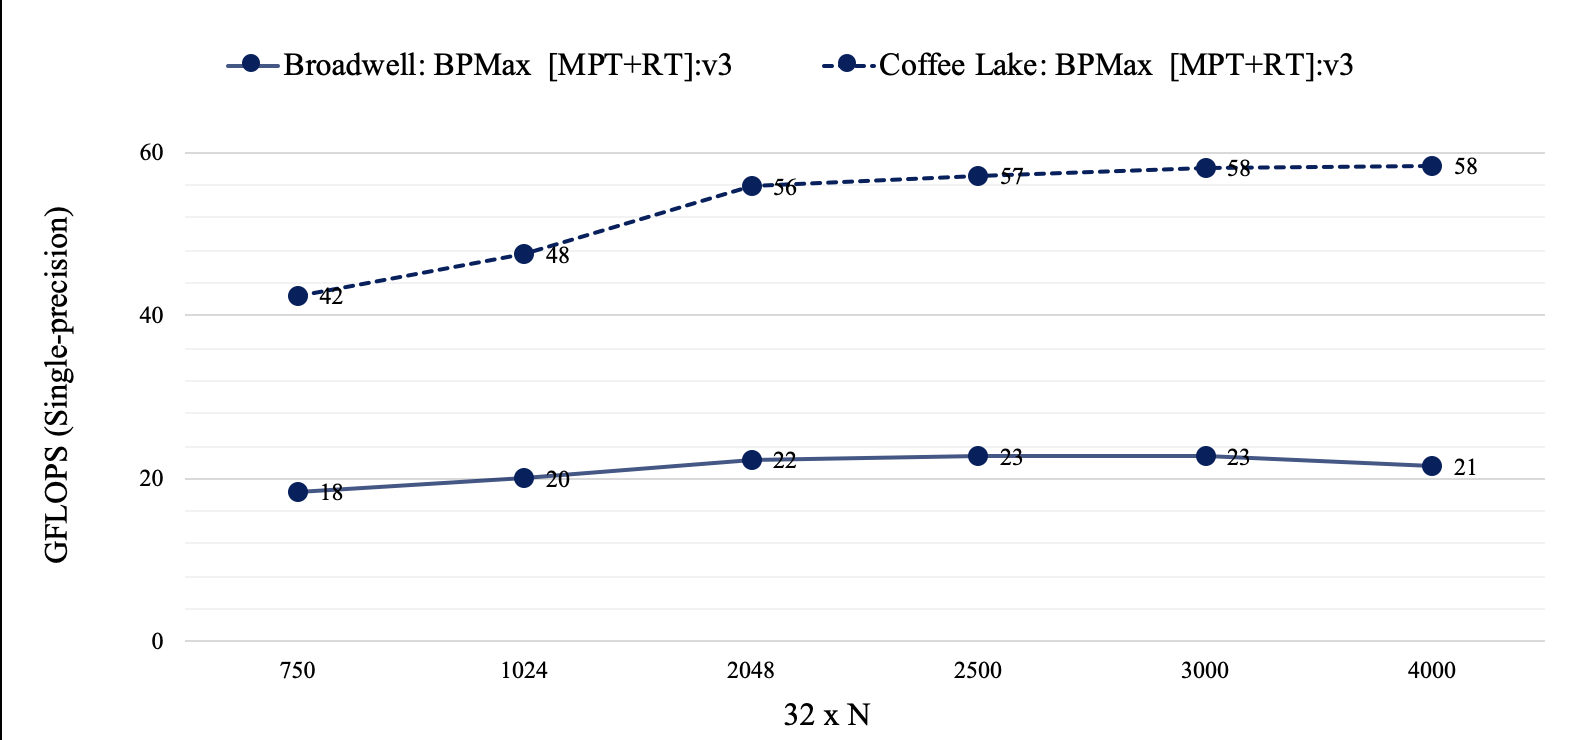
\includegraphics[scale=0.38, trim=5 5 5 5,clip]{content/figures/bpmax_single_core.png}}
\caption{BPMax Single Core Performance}
\label{fig:st_performance_analysis_bpmax}
\end{figure}

\subsubsection{Multi-Core Performance}

\begin{figure*}[htbp]
\centerline{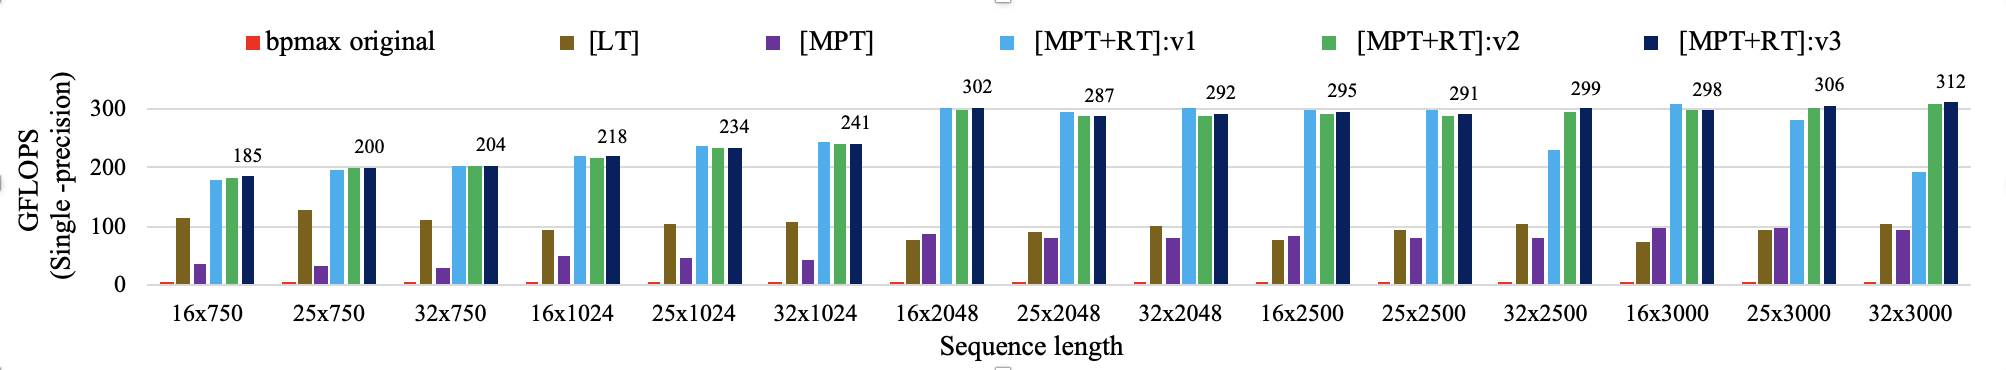
\includegraphics[width=\textwidth,scale=1.00, trim=5 5 5 5,clip]{content/figures/bpm_performance_new_tile.png}} 
\caption{BPMax performance comparison on Coffee Lake}
\label{fig:bpm_performance}
\end{figure*}


\begin{figure*}[htbp]
\centerline{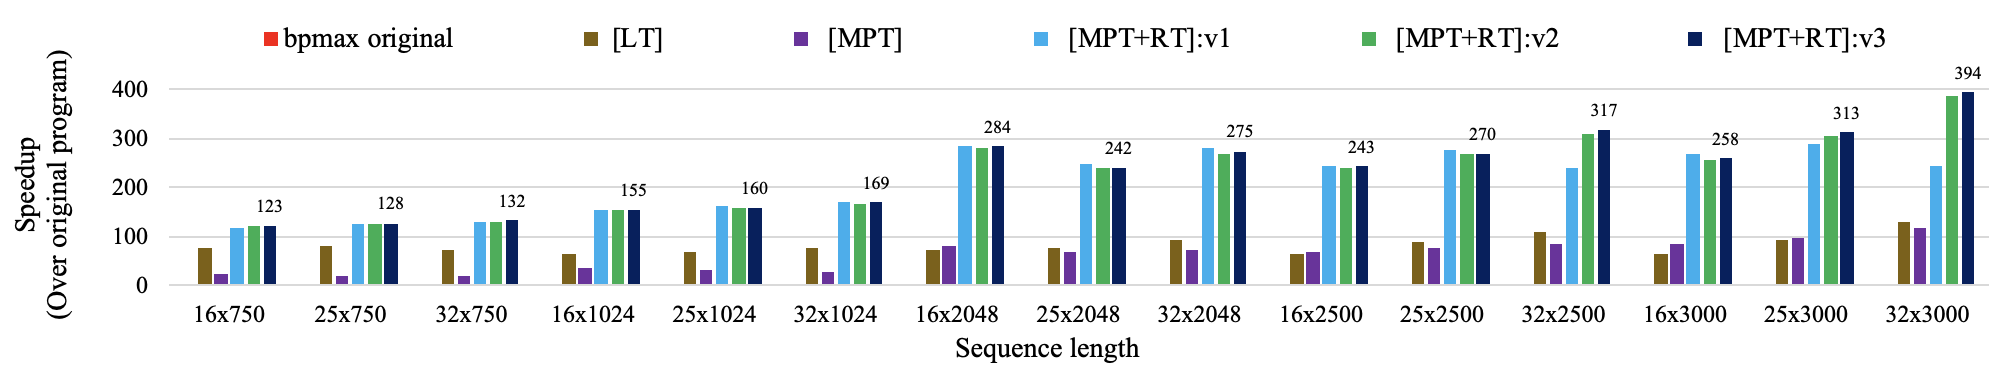
\includegraphics[width=\textwidth,scale=1.00, trim=5 5 5 5,clip]{content/figures/bpm_speed_up_new_tile.png}} 
\caption{BPMax speedup comparison on Coffee Lake}
\label{fig:bpm_speed_up}
\end{figure*}
Figure~\ref{fig:bpm_performance} and ~\ref{fig:bpm_speed_up} show the performance improvements and speedup of various versions of BPMax program on Coffee Lake with $8$ threads. We use the original implementation (BPMax original) as the reference highlighted in red. 
The performance and speedup with the best optimized previous version \cite{Mondal2021} ([LT]) is highlighted in brown. [LT] earlier achieved  $100\times$ speedup for longer sequence lengths. It can be observed that that [LT] only saturates fraction of the machine peak. The last four data points use different versions of the current work. 

The first data point [MPT] with our new implementation is highlighted in purple, which does not employ the register tiling but uses mono-parametric tiles for the second-level tile. It employs similar program transformations like all the versions of the [MPT] to improve data locality for each tile. We observe that a mono-parametric tile size of 192 works better across all the inputs. [MPT] shows no performance improvement over [LT] because the best tile size was not long enough for effective vectorization. However, [MPT] is essential for applying register tiling.

We have experimented with three types of data-transformation techniques with our register-tiled code. \textbf{[MPT+RT]:v1} performs best when the memory footprint is low. As the memory footprint increases, it performs poorly. There is no significant differences between the \textbf{[MPT+RT]:v2} and \textbf{[MPT+RT]:v3}. However, the \textbf{[MPT+RT]:v3} performs consistently well across all the inputs. Figure~\ref{fig:bpm_performance} and~\ref{fig:bpm_speed_up} show the performance and speed up achieved by the \textbf{[MPT+RT]:v3}. It attains a peak performance of $53\%$ of the roofline machine peak on Coffee Lake, about $400\times$ faster than the base program. Figure~\ref{fig:roof_line_coffee_lake} shows the CPU usage of different parts of the BPmax program. We observe that $72\%$ of the program's execution time (139s/187s) is spent in the register-tiled kernel, which achieved $82\%$ of the roofline peak. The remaining $30\%$ of the program spent significant time in vectorized code and memory initialization. However, it is important to note that additional work is done when a mono-parametric tile is filled with max-plus identity values corresponding to the triangular tiles from the edge of the inner triangle. These additional computations over the identity elements are excluded from the GFLOPS computation reported in the figures. Our polyhedral compilation scripts and source codes are available in the GitHub repository\footnote{https://github.com/chiranjeb/BPMaxCPU}.
